%!TEX root = foo-thesis.tex


\chapter{Implementation}

\section{Used Framework and Libraries}

\begin{figure}[htbp]
  \centering
  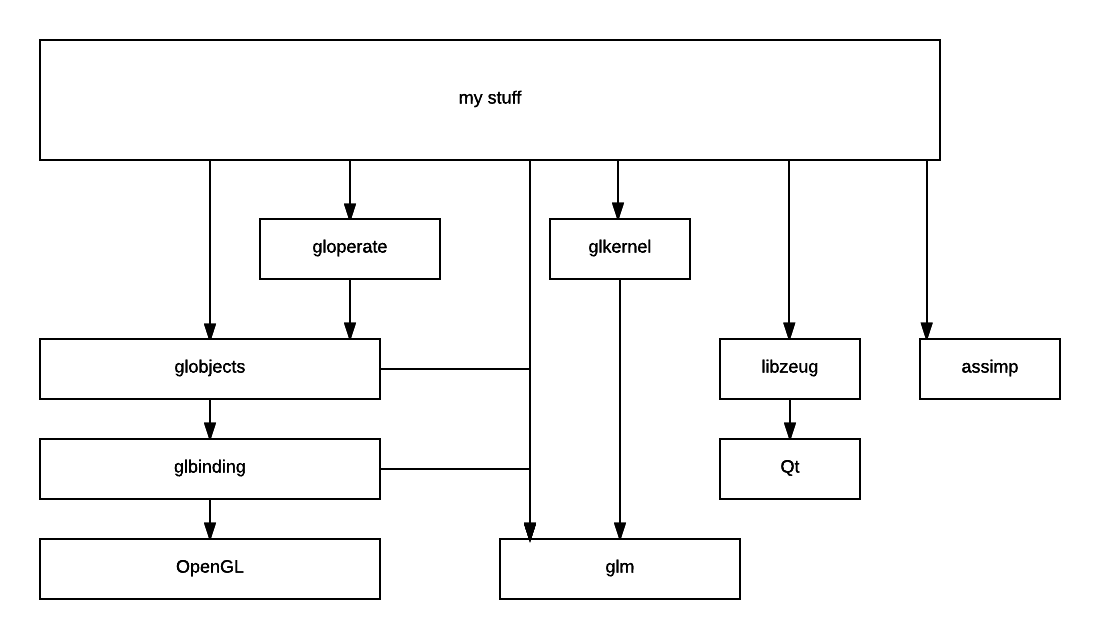
\includegraphics{graphics/Architecture}
  \caption{svg image}
\end{figure}

\begin{outline}
\1 gloperate as framework
    \2 uses qt
\1 libzeug provides GUI elements
\1 globjects as an object-oriented abstraction over OpenGL
\1 glbinding provides OpenGL bindings, directly called sometimes
\1 GLM provides math and easier interaction with the OpenGL API
\1 no further relevance for this thesis:
    \2 assimp for model loading
    \2 glkernel provides kernels for our SSAO implementation
\end{outline}

\section{Rendering Pipeline Overview}
\begin{outline}
\1 would be much the same as the concept pipeline...
\1 show what's compute shader and what not?
\1 it's basically lighting plus
    \2 g-buffer generation
    \2 shadowmap which is part of the RSM,
    \2 SSAO
    \2 deferredshading
    \2 srgb and HDR.
    \2 all of this is not
\1 model loading?
\1 kernel generation?
\end{outline}


\section{RSM Generation and VPL Sampling}
\label{sec:impl:rsmAndVplSampling}
\begin{outline}
\1 use the same code for RSM generation as for G-Buffer generation with only slight modifications:
\1 don't use normalmaps as the triangle normals are sufficient
\1 instead of individual texture lookups, we use the material's average color as diffuse color as suggested by \citet{hedman2016sequential} to avoid high-frequency color changes to affect the outcome.
\1 we re-use RSM as shadowmap
    \2 usually, one might want to decouple this since they likely need different resolutions/cascading schemes etc. One could also render the RSM with a less detailed version of the scene. Since we had no culling and LOD implemented, we were bottlenecked on geometry complexity and chose to do this in one pass.
    \2 we use variance shadowmapping. so we add the variance buffer if we're rendering an RSM, and disable another buffer (non-face normals).

\1 with a compute shader, we sample the RSM in a regular pattern and write VPLs into a buffer
\1 VPLs are position, normal, color
\1 we prepare a second buffer with a single vec4 with position in the first three values and normal packed into the last value.
\1 we do that since the ISM rendering (Section~\ref{sec:impl:ismRendering}) and light list calculation (Section~\ref{sec:impl:clusteredShading}) do not need color and especially ISM rendering reads several VPLs per point, using a lot of bandwidth.
\1 Because of the regular sampling, the noise produced during interleaved shading (Section~\ref{sec:impl:interleavedShading} or only results? there was a paper that sorts VPLs to avoid the noise...) is more structured. To help with that, we permutate the VPL order with a random permutation computed on CPU
\end{outline}


\section{ISM Rendering}
\label{sec:impl:ismRendering}

\begin{outline}
\1 Our ISM rendering normally draws all the geometry in the scene.
\1 In the tessellation control shader, the tesselation levels are determined depending on the triangle size.
\1 The tessellation evaluation shader does nothing besides correctly interpolating the triangle's vertices.
\1 The geometry shader, which now recieves a small (tesselated) triangle, computes the point data
\1 i.e. position: center of triangle, radius: distance of center to farthest triangle vertex, normal: the face normal taken from the original, non-tessellated triangle.

\1 the geometry shader then calculates a random VPL ID. We used the point's barycentric coordinate inside its triangle and the triangle's primitive ID to seed the random number generator, as both values are readily available and coherent between frames.
\end{outline}

\subsection{Point Rendering with Splatting}
\1 two approaches:

\1 either the geometry shader itself reads the VPL with the index it determined, projects the point according to the VPL's data, sets gl\_PointSize to the projected size, and emits a vertex.
\1 also, output mode is points.

\1 \citet{Marroquim:2007:reconstruction} actually works with single-pixel ``splats''. since in this case we're not depending on the hardware rasterizer for good performance, this inspired the following approach:

\subsection{Point Rendering with Pull-Push Postprocessing}
\1 instead of splatting, the geometry shader puts points into buffer
\1 one buffer per VPL for stability
\1 buffers index marks the first VPL to try
\1 then, per point in each buffer, starting with the respective VPL, we test a fixed number of VPLs (e.\,g. 16) and collect up to 4 that pass culling tests.
\1 specifically, backface culling and points that are located behind the VPL, i.\,e. not in the hemisphere pointing along the VPL's normal.
\1 we then render the point as a single pixel into the 4 collected VPLs.

\todo{part of this into concept}


\1 hole mitigation
\1 when splatting, the quality difference improvement achieved with an additional pull-push algorithm compared to slightly larger splats seemed not worth the performance impact, therefore we chose to simply enlarge all splats a bit.
\1 when using compute shaders, we need pull-push by design.
\end{outline}

\todo{explain pullpush implementation}

\section{Interleaved Shading with Compute Shaders}
\label{sec:impl:interleavedShading}
\begin{outline}
\1 often, de-interleaving is implemented by splitting the G-buffer into several smaller G-buffers, each containing all pixels with the same sample set \cite{segovia2006non}. Each G-buffer is processed with its respective sample set, and then the buffers are re-interleaved into a large G-Buffer again.

\1 instead, we do this in a single pass. compute shaders are launched so that each invocation processes one pixel, and invocations within a work group process the same VPL set.
\1 \ref{lst:???}?
\1 diagram of the pixels. \ref{fig:impl:pixels} explain this. we still do coherent VPL processing.
\1 more explanation on id calculation
\1 reasons for single pass? easier to implement. latency covering? less bandwidth? less memory. compared to interleaving via shared memory, occupancy and scales to 8x8.
\1 potential downside is the scattered read compared to coherent read when doing the split. but, bottleneck is lookups in the VPL buffer and the respective shadowmaps in the main loop, as well as ALU operations, so this noe-time lookup doesn't have any impact. maybe completely latency covered or workgroups are distributed in a way that the reads are still cache-coherent.
\1 in fact, any attempts to do coherent reads did not result in speedups.

\1 Since only a subset of all samples is processed per pixel and this subset repeats every four pixels, this process results in structured noise (see Figure \ref{fig:???} or this figure in concept?)
\1 therefore, geometry-aware blur similar to \citet{laine2007incremental}. doesn't smooth over edges. See code snippet \ref{listing:???}. every pixel has all the information now ideally.

\1 VPL shuffling helps a great deal! See Figure \ref{fig:impl:shuffling}
\end{outline}

\section{Clustered Deferred Shading}
\label{sec:impl:clusteredShading}

\begin{outline}
\1 we use 128 pixels as screen-space tile width and 16 depth slices. We also use an optimization proposed by \citet{persson::2013::practical} and use a larger near cluster for better depth slice utilization.

\1 we do not use explicit bounds, since we expect only small gains by that. although it might result in larger gains, we have have not implemented using normals for clustering yet.
\1 \citet{???practical} do culling on the CPU. they have small radii and can therefore quickly determine the clusters that are reached by a certain light.
\1 we have infinite light radii and therefore lots of clusters per light. therefore, we can expect to cull maybe half the lights and not the majority.
\1 therefore, we decided to iterate over all lights per used cluster, as opposed to iterate over reached clusters per light.
\1 the more uniform control flow of this approach as also better suited to GPUs.


\1 three phases, each corresponding to one dispatch compute call:
\1 clustering
    \2 each work group processes one tile and has one 16 bool array which indicates which depth slices in that tile are used.
    \2 for each fragment, set the corresponding bool to true. no synchronization needed.
    \2 since the work group size is limited, we set it to 128 and let each invocation iterate through 128 pixels in the tile to cover all pixels.
    \2 per work group, count the number of used slices
        \3 we use the first 16 threads in the work group and atomic adds, but one could just as well let one thread do it serially, it doesn't matter.
    \2 then it adds the number of used depth slices to one global atomic counter. the glsl function to do this returns the value of the counter before the addition.
    \2 this way, each workgroup ``allocates'' some space in the list of used clusters. it then writes an id for each cluster into that list.
\1 calculating light lists
    \2 one invocation per used cluster.
    \2 calculate world-space corners of that cluster.
    \2 show some code? but it's really ugly...
    \2 for each light
        \3 if any corner is inside the illuminated hemisphere, add the light to this cluster's light list.
    \2 we simply allocate the maximum space for this.
        \3 for full HD / 128px tiles = 135 tiles, * 16 depth slices = 2160 light lists, * 1024 vpls = 2160k indices, * 2 bytes per index makes 4mb.
        \3 we thought it's unneccessary to cut that down.
        \3 by a (conservative) estimate of four used depth slices per tile on average, (plus possibly runtime checks to allocate more space when running over that limit), on could reduce this to 1MB with little implementation effort.
        \3 compacting the light lists themselves is probably not worth it due to implementation complexity and performance penalty
        \3 since we expect to cull roughly half the lights, the potential saving by compacting the light lists is only 50\% anyways.
\1 shading
    \2 during shading, when processing a pixel, the pixel's cluster is first determined and only the lights of this cluster's light list are processed.
    \2 we use a very basic approach to combine this with interleaved shading: of all lights in the light list, each pixels gets an equally sized fraction. while this might lead to adjacent pixels processing overlapping sets of lights if they are in different clusters, they are either in clusters near to each other in which case the light lists are probably quite similar, or they are in clusters seperated from each other so the geometry-aware blur wouldn't consider them anyway.

\end{outline}
